% !TEX TS-program = pdflatex
% !TEX encoding = UTF-8 Unicode

% Example of the Memoir class, an alternative to the default LaTeX classes such as article and book, with many added features built into the class itself.

\documentclass[10pt,twocolumn,article]{memoir} % for printing/viewing for text proofreading

%documentclass[12pt,letterpaper]{memoir} % closer to real thesis format
%\settypeblocksize{9in}{6.5in}{*}
%\setlrmargins{1in}{*}{*}
%\setulmargins{1in}{*}{*}

\usepackage[utf8]{inputenc} % set input encoding to utf8

%\usepackage{times}

\usepackage[sc]{mathpazo}
%\renewcommand{\familydefault}{ppl}

\usepackage[cmex10]{amsmath}
\usepackage[kerning]{microtype}
\usepackage{cite}

\usepackage{enumitem}
\usepackage{graphicx}
\usepackage{booktabs}

\usepackage{xspace} % fix trailing spaces after abbreviation macros

\setlist{nolistsep} % or \setlist{noitemsep} to leave space around whole list

% My macros
\newcommand{\figref}[1]{Figure~\ref{#1}}
\newcommand{\tableref}[1]{Table~\ref{#1}}
\newcommand{\TES}{{\small TES}\xspace}
\newcommand{\He}[1]{He#1\xspace}
%\newcommand{\He4}{}

\title{A 350 GHz Video Imaging System}
\author{Dan Becker}
%\date{} % Delete this line to display the current date

%%% BEGIN DOCUMENT
\begin{document}

\maketitle

%%%\begin{abstract}
%%%Passive millimeter-wavelength video imaging systems hold promise for detection of security threats at a distance, such as including suicide bomb belts and maritime threats in fog.
%%%Achieving optimal noise and optical performance for these system requires large numbers of cryogenic millimeter-wavelength radiation detectors. Large-format arrays of superconducting Transition Edge Sensor (TES) bolometers have been proven to meet requirement for both noise and number of detectors.
%%%We are developing a video- rate millimeter-wavelength imaging system using 1004 TES bolometers as detectors.
%%%This demonstration system detects is intended to have photon-noise-limited performance, and will be used to investigate phenomenology of passive millimeter-wavelength video images, with the goal of identifying what performance tradeoffs can be made when building a deployable system.
%%%It observes light in a 10\% band centered at 350 GHz, and is designed to take video images at distances ranging from 16 m to 28 m.
%%%When operating at 16 m, the resolution is 1 cm over a 1 m by 1 m field of view.
%%%The system is predicted to take video images with a noise equivalent temperature difference (NETD) of 100 mK at 20 frames per second.
%%%This thesis describes the design and implementation of this system, as well as imaging results from the first 251-detector subarray to be installed.
%%%\end{abstract}

%\tableofcontents* % the asterisk means that the contents itself isn't put into the ToC

%%%(211 words, 350 allowed)

\chapter{Introduction}\label{c:intro}

\chapter{System Specifications, Challenges and Solutions}\label{c:specs}

\chapter{TES Bolometer Theory}\label{c:tes}

\chapter{System Design Overview}\label{c:sys-design}

\section{Cryostat Design}\label{s-cryo-design}

The cryostat for the 350~GHz Imager was designed with the goals of simplicity, reliability and turn-key automated operation.
Highly reliable and easy-to-use cryogen-free mechanical cryocoolers are available from many vendors, but these cryocoolers are seldom capable of reaching temperatures below 2.5~K.
To reach sub-Kelvin temperatures a second refrigeration stage is required, which in our case is a He-4 sorption refrigerator.
The He-4 sorption refrigerator is based on a proven design and its use can easily be automated.
Three temperature stages within the cryostat are provided in order to provide intercepts for heatsinking wiring and other objects that are thermal connected to room temperature. 
The result is a cryogen-free cryogenic system that can be controlled remotely and has run for over 1000 (xxx) hours.

The cryostat itself was designed and built by Precision Cryogenics (xxx give addr and other info?) to specifications provided by the 350~GHz Imager team.
\figref{fig:cryo-cutaway} shows a cutaway view of the cryostat, and \tableref{tab:temp-optical-load} lists the temperatures typically reached by different parts of the cryostate during operation when the cryostat is open optically.
The cryostat has two main parts: a cylinder containing both the PTC and the He4 sorption refrigerator, and a box located at the bottom of the cylinder which contains temperature intercept plates and the focal plane.
There are three temperature stages, the ``90~K'' Cold Plate, the ``4~K'' Cold Plate, and the Focal Plane.
The PTC 1st stage is connected to the ``90~K'' Cold Plate by a tube of Al xxx and a set of xxx copper braids.
The combination of this long thermal path with the high heat load on the optical filters sunk to the ``90~K'' stage explains the 45~K temperature differential between the ``90~K`` cold plate and the PTC 1st stage.
The PTC 2nd stage is connected to the ``4 K'' Cold Plate by a large (xxx by xxx) cylinder of xxx Cu\footnote{This cryostat was originally designed to work with a different cryocooler. The PTC currently installed had a shorter distance between the 1st and 2nd stages, neccesitating the Cu cylinder to take up this extra space}, followed by tube of OFHC (xxx check) Cu followed by a set of xxx copper braids.
The Cu tube is broken into two halves, and the condensation plate (see below) of the sorption fridge is clamped between these two halves. The ``90 K'' Cold Plate is stood off from the cryostat vacuum jacket by four carbon-fiber standoffs. (xxx check with Bob S). The ``4~K'' Cold Plate stands off from the ``90 K'' Cold Plate by 12 (xxx check) supports made of G-10.

The first two temperature intercept stages are provided by a Cryomech PT407 Pulse Tube Cryorefrigerator (xxx reference company info).
The PT407 has two cooling stages.
The first stage has 25~W of cooling power at 55~K while the second stage has 0.7~W at 4.2 K.
Our PT407 uses a remote motor, so that the cold head attached to the cryostat has no moving parts, minimizing vibration of the cryostat.
Vibration of the cryostat can lead to microphonic pickup either directly in the detectors themselves or in the readout circuitry, leading to much higher detector noise.

\begin{figure*}[th]
\centering
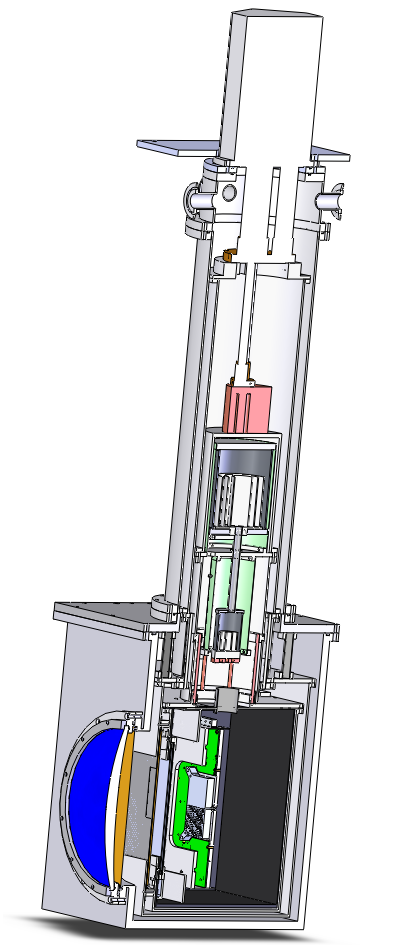
\includegraphics[width=0.5\textwidth]{images/cryostat-cutaway.png}
\caption{Cutaway view of the 350 GHz Imager. xxx should probably label things here.}
\label{fig:cryo-cutaway}
\end{figure*}

\begin{table*}[ht]
\centering
\caption{Temperatures Reached Under Optical Load xxx check all when temps have settled xxx should I add temps when closed optically?}
\label{tab:temp-optical-load}
\begin{tabular}{l r}
\toprule
Temperature Stage &  Temperature (K)\\
\midrule
PTC 1st Stage Cold Head 			& 52 \\
PTC 2st Stage Cold Head 			& 3.6 \\
Cryostat ``50 K'' Cold Plate 		& 96 \\
Cryostat ``4 K'' Cold Plate 			& 6.4 \\
Sorption Fridge Condensation Plate 	& 3.8 \\
Focal Plane 						& 0.970 \\
\bottomrule
\end{tabular}
\end{table*}

There are many options for reaching temperatures below the $\sim$1.2~K transition temperature of our \TES detectors: dilution refrigerators, adiabatic magnetization refrigerators, pumped \He4 baths, \He3 and/or \He4 sorption refrigerators.
We chose a \He4-sorption fridge because of both it's low and cost ease of operation compared to other solutions, and the fact that the typical base temperatures under no load of $sim$700~mK is well-matched to our application.
A  \He4-sorption fridge works by using a charcoal adsorber to pump on a bath of liquid \He4, reducing the \He4 boiling point and thus the temperature of the bath.
The \He4 is contained withing a sealed reservoir so that the refrigerator acts as a closed system requiring no \He4 replenishment. 
While \He4-sorption fridges are commercially available, our team choose to design and build a custom fridge based on a design that has been proven in many astronomical applications (xxx ref).

\figref{fig:he4sorp} shows a schematic depiction of the 350~GHz Imager's \He4-sorption refrigerator.
The entire refrigerator is filled with xxx moles of \He4 gas, giving a pressure of xxx psi at room temperature.
In normal operation the heat switch between the charcoal pumping chamber (``pump'') and the \He4 condensation plate is closed, keeping the charcoal as cold as possible in order to adsorb as much \He4 as possible, keeping the temperature of the cold plate as low as possible.

Cycling the refrigerator requires xxx steps. First the heat switch opened.
The \He4-sorption refrigerator uses a \He4 gas-gap heat switch manufactured by Chase Cryogenics (xxx ref), which requires 5 minutes of waiting time in order for the switch to fully open.
Second, the pump is heated by applying xxx W of power via a xxx Ohm power resistor.
This power is applied until the temperature of the pump reaches 40 K, which is high enough to drive nearly all of the adsorbed \He4 off of the charcoal.
Third, the power to the pump is turned off.
Once the temperature of the condensation plate falls below the boiling point of \He4, \He4 will begin to condense on it's walls, dripping into the \He4 condensation pot (``pot'').
Fourth, once the temperature of the pot has fallen to 4.0~K, the heat switch is turned back on. This cools the pump, allowing \He4 to again adsorb onto the charcoal, which has the effect of pumping strongly on the pot, and cooling the \He4 contained there to the base temperature of $\sim$ 970~mK under optical load.

\chapter{Detector Design}\label{c:det-design}

\chapter{Focal Plane Design}\label{c:fp-design}

\chapter{Detector Characterization}\label{c:det-char}

\chapter{Imaging}\label{c:imaging}

\chapter{Vocab}

Placeholder for terms

\begin{description}
\item[``90~K'' Cold Plate]
\item[``4~K'' Cold Plate]
\item[Sorption Fridge]
\item[350~GHz Imager]

\end{description}

\end{document}
